\section{Visualization}

In order to create a visualization of the algorithms described in the previous sections, a 3D model of the floor plan of the museum was created. First, this floor plan is converted into an SVG image so it can easily be altered in Python. Working this way makes it possible to dynamicly create an HTML page showing the SVG floor plan and the currently analyzed frame along with the detected paintings. Because some operations need a lot of processing power, two seperate processes are spawned. One process handles the painting detection and room prediction, the other one handles the visualization of the HTML page in a webview. One of the major points of attention during the creation of the visualization was performance, hence the HTML file is never written to disk in order to bypass the I/O operations. Therefor interprocess communication is used to send the HTML page to the second process. When this process receives an HTML page, it can be visualized in the webview. An example of this webview is shown in \figureref{fig:webview}. Besides showing the floor plan and the image, other information is shown as well. This includes information about the predicted room, which is also visualized in red on the floor plan, a probability for this prediction, the currently processed video's name and the currently analyzed frame.

\begin{figure}
    \centering
    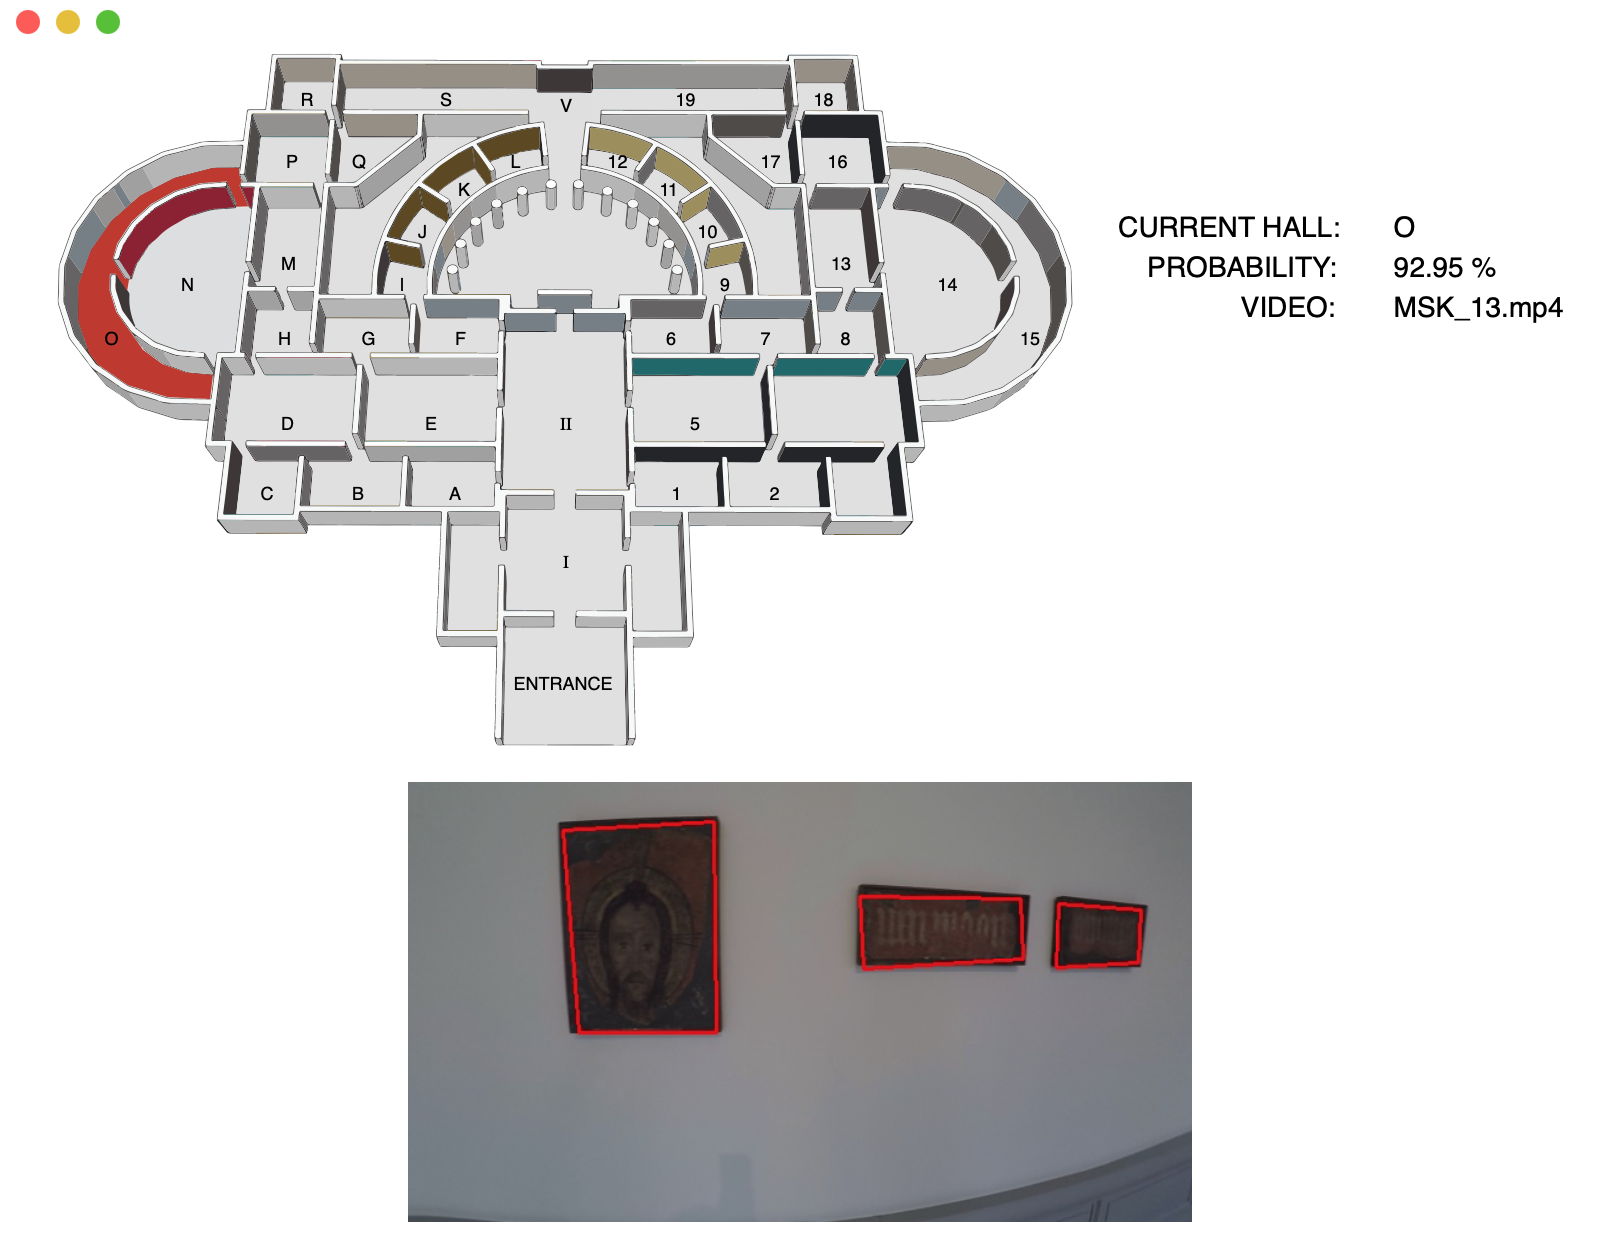
\includegraphics[width=0.7\linewidth]{visualization.png}
    \label{fig:webview}
    \caption{Modern visualization of the floor plan}
\end{figure}
